\subsection{Merge Sort}

\begin{table}[h]
	\begin{center}
		\begin{tabular} { >{\centering\arraybackslash}m{3cm} | >{\centering\arraybackslash}m{3cm} | >{\centering\arraybackslash}m{2cm} | >{\centering\arraybackslash}m{2cm} }
			\hline
			\textbf{Language} & \textbf{\# of elements}	& \textbf{Time(s)} & \textbf{Ratio}  \\ \hline
			C\#					& 10'000		& 0.005 		& 1:1 		\\ \hline
			Java				& 10'000		& 0.067 		& 1:13.4 	\\ \hline
			Python				& 10'000		& 0.67	 		& 1:134 	\\ \hline
		 \\ \hline
			C\#					& 100'000		& 0.092 		& 1:1 		\\ \hline
			Java				& 100'000		& 0.155 		& 1:1.7 	\\ \hline
			Python				& 100'000		& 88.672 		& 1:963 	\\ \hline	
		\end{tabular}
	\end{center}
	\caption{Results from sorting 10'000 and 100'000 elements using Merge Sort.}
	\label{table:merge_sort}
\end{table}

Since the runtime for Python was already over the one minute mark with just 100'000 elements (see Table \ref{table:merge_sort}) I decided not to test one million elements with Python. Instead I tested C\# and Java with one million elements and compared the runtimes with one hundred thousand elements in Figure \ref{fig:merge_sort_csharp_java}.

As Table \ref{table:merge_sort} illustrates, the ratio for Python seemed to get worse and worse in relation to the number of elements sorted. 

\begin{figure}[h]
	\centering
	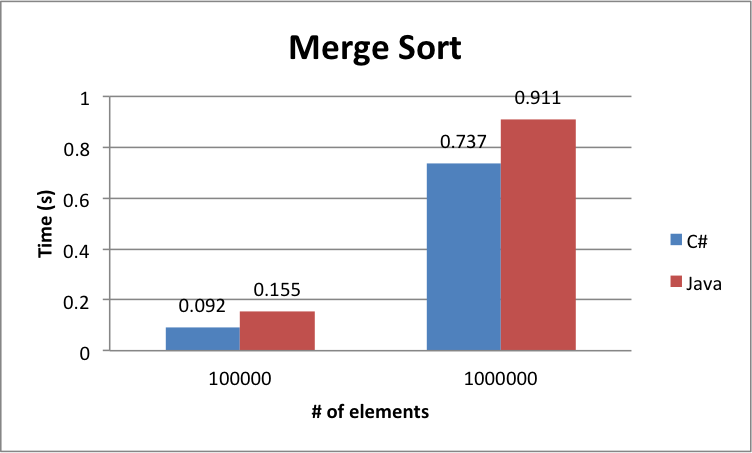
\includegraphics[width=0.6\textwidth]{chapters/media/merge_sort_csharp_java.png}
	\caption{Time difference between using 100'000 elements and a million.}
	\label{fig:merge_sort_csharp_java}
\end{figure}

C\# still outperforms Java when run under the .NET environment. But the gap between them seemed to narrow the more elements were added. I attempted to run Java under its native environment, and it  outperformed C\# (see Figure \ref{fig:merge_sort_csharp_java_native}). 

Java run under .NET is about equal to C\# when it comes to memory management as seen in Figure \ref{fig:merge_sort_memory}. 

\begin{figure}[h]
	\centering
	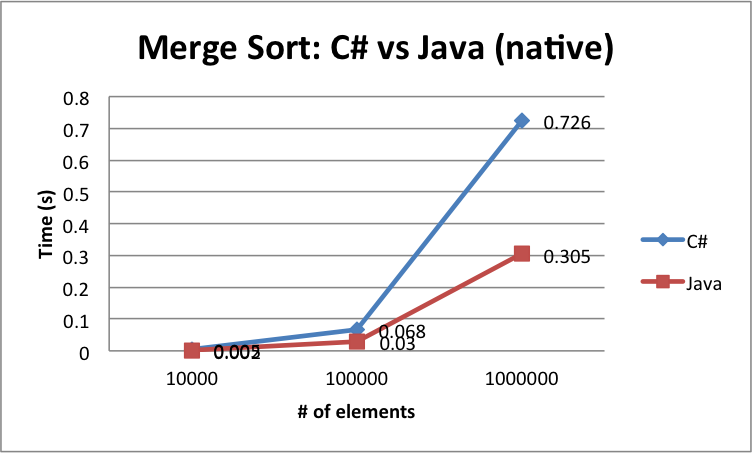
\includegraphics[width=0.6\textwidth]{chapters/media/merge_sort_csharp_java_native.png}
	\caption{Comparing Java and C\# when both are run in their respective native environments.}
	\label{fig:merge_sort_csharp_java_native}
\end{figure}

\begin{figure}[h]
	\centering
	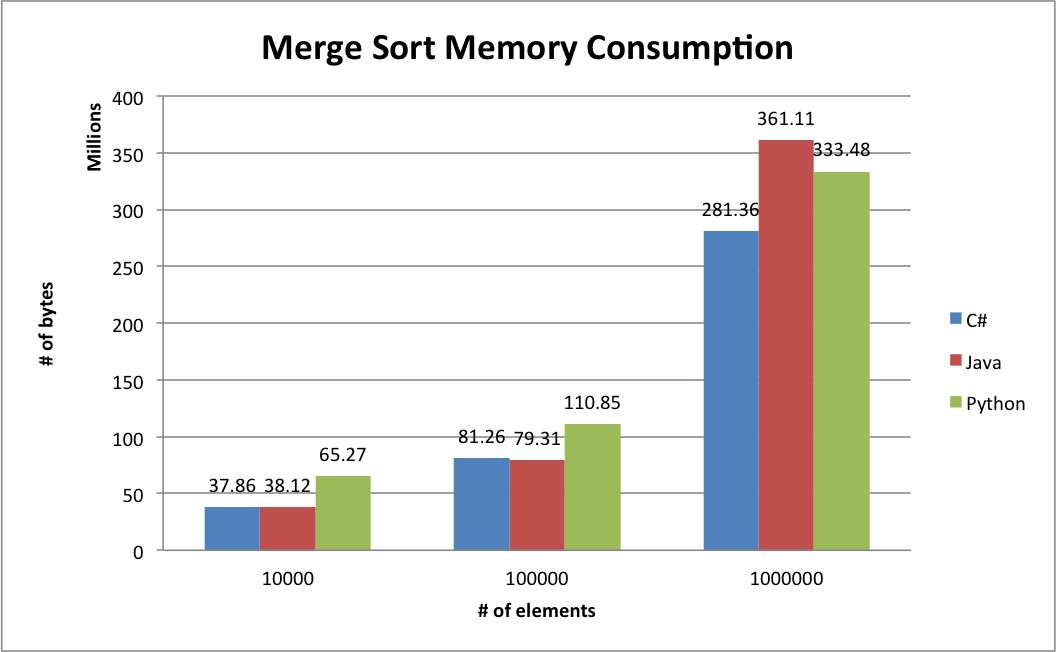
\includegraphics[width=0.6\textwidth]{chapters/media/merge_sort_memory.png}
	\caption{Comparing Java and C\# when both are run in their respective native environments.}
	\label{fig:merge_sort_memory}
\end{figure}